\chapter{Backtracking}

\section{Regular Expression Matching} %%%%%%%%%%%%%%%%%%%%%%

\subsubsection{Description}
Implement regular expression matching with support for \fn{'.'} and \fn{'*'}.

\fn{'.'} Matches any single character.
\fn{'*'} Matches zero or more of the preceding element.

The matching should cover the entire input string (not partial).

Some examples:
\begin{Code}
isMatch("aa","a") → false
isMatch("aa","aa") → true
isMatch("aaa","aa") → false
isMatch("aa", "a*") → true
isMatch("aa", ".*") → true
isMatch("ab", ".*") → true
isMatch("aab", "c*a*b") → true
\end{Code}

\subsubsection{Solution}

\begin{Code}
public boolean isMatch(String s, String p) {
    if (p.isEmpty()) {
        return s.isEmpty();
    } else if (p.length() == 1) {
        return s.length() == 1 && isEqual(s, p);
    } else if (p.charAt(1) != '*') {
        return s.length() > 0 && isEqual(s, p) && isMatch(s.substring(1), p.substring(1));
    } else {
        if (s.length() > 0 && isEqual(s, p)) {
            return isMatch(s, p.substring(2)) || isMatch(s.substring(1), p);
        } else {
            return isMatch(s, p.substring(2));
        }
    }
}

private boolean isEqual(String s, String p) {
    return s.charAt(0) == p.charAt(0) || p.charAt(0) == '.';
}
\end{Code}

\newpage

\section{Wildcard Matching}

\subsubsection{Description}
Implement wildcard pattern matching with support for \fn{'?'} and \fn{'*'}.

\fn{'?'} Matches any single character.
\fn{'*'} Matches any sequence of characters (including the empty sequence).

\begin{Code}
Some examples:
isMatch("aa","a") → false
isMatch("aa","aa") → true
isMatch("aaa","aa") → false
isMatch("aa", "*") → true
isMatch("aa", "a*") → true
isMatch("ab", "?*") → true
isMatch("aab", "c*a*b") → false
\end{Code}

\subsubsection{Solution}
\begin{Code}
public boolean isMatch2(String s, String p) {
    int is = 0, ip = 0, ks = -1, kp = -1;

    while (is < s.length()) {
        if (ip < p.length() && (s.charAt(is) == p.charAt(ip) || p.charAt(ip) == '?')) {
            is++;
            ip++;
        } else if (ip < p.length() && p.charAt(ip) == '*') {
            ks = is;
            kp = ip;
            ip++;
        } else if (kp != -1) {
            is = ++ks;
            ip = kp + 1;
        } else {
            return false;
        }
    }

    for ( ; ip < p.length() && p.charAt(ip) == '*'; ip++);
    return ip == p.length();
}
\end{Code}

\newpage

\section{Letter Combinations of a Phone Number}

\subsubsection{Description}
Given a digit string, return all possible letter combinations that the number could represent.

A mapping of digit to letters (just like on the telephone buttons) is given below.

\begin{center}
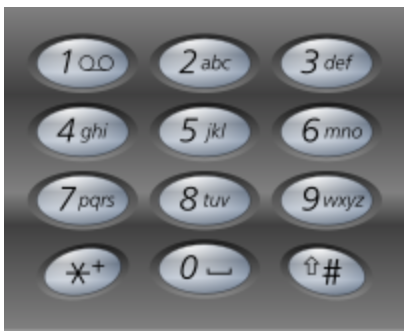
\includegraphics[width=150pt]{phone.png}\\
\figcaption{Phone Keyboard}\label{fig:phone-keyboard}
\end{center}

\textbf{Input:} Digit string \code{"23"}

\textbf{Output:} \code{["ad", "ae", "af", "bd", "be", "bf", "cd", "ce", "cf"]}.

\subsubsection{Solution}

\begin{Code}
private final String[] ARR = {
        "", "", "abc", "def", "ghi", "jkl", "mno", "pqrs", "tuv", "wxyz"
};

public List<String> letterCombinations(String digits) {
    List<String> list = new LinkedList<>();
    if (!digits.isEmpty()) {
        helper(digits, 0, list, "");
    }
    return list;
}

private void helper(String digits, int start, List<String> list, String s) {
    if (start >= digits.length()) {
        list.add(s);
        return;
    }
    int n = digits.charAt(start) - '0';
    for (char c : ARR[n].toCharArray()) {
        helper(digits, start + 1, list, s + c);
    }
}

public List<String> letterCombinations2(String digits) {
    LinkedList<String> queue = new LinkedList<String>();
    if (digits.length() == 0) {
        return queue;
    }

    Queue<String> next = new LinkedList<>();
    queue.add("");

    for (int i = 0; i < digits.length() && !queue.isEmpty(); ) {
        String s = queue.poll();
        int n = digits.charAt(i) - '0';
        for (char c : ARR[n].toCharArray()) {
            next.add(s + c);
        }
        if (queue.isEmpty()) {
            queue.addAll(next);
            next.clear();
            i++;
        }
    }
    return queue;
}
\end{Code}